\section{Evaluation}
\label{sec:experiment}


%In this paper, our task is to tackle commonsense reasoning problem in stories. 
%Given SCT as evaluation set, we can use any source data to learn human commonsense knowledge and reasoning ability. 
%We suppose the validation data has information leak for test set. The most classification methods which training or fine tuning with SCT validation set may learn the bias leak features, rather than commonsense reasoning ability
We first introduce baseline methods to be evaluated against as well as
the datasets we used.
Then we present a preliminary analysis on the ROCStories dataset to invalidate
previous approaches that train or fine-tune their models on the validation
set and we reconstruct a new dataset for training. Finally we conduct a comprehensive
evaluation of the competing methods to verify the effectiveness of our simplification method and 
the structured knowledge we incorporate.

%In this paper, our task is to tackle commonsense reasoning problem in stories. 
%Given SCT as evaluation set, we can use any source data to learn human commonsense knowledge and reasoning ability. 
%We suppose the validation data has information leak for test set. The most classification methods which training or fine tuning with SCT validation set may learn the bias leak features, rather than commonsense reasoning ability(\secref{sec:dataset}). We suggest to use a larger corpus with negative ending generated automatically. We also show our model parameter details in \secref{sec:details}, the comparison result with analysis in \secref{sec:result} and ablation study is in \secref{sec:ablation} .
\subsection{Baselines and Our Methods}
\label{sec:baselines}
%\KZ{Which version of ConceptNet did we use?}
%We evaluate our methods against two group of baseline methods.
%\KZ{Actually our methods shouldn't be eval against the other baselines,
%rather they should be ``added'' on to the other baselines. There are
%two types of baselines. The first type is pretrained model, and
%we need to explain why our simplification and CE methods are better 
%applied to this type of models.}
%First, as mentioned in ~\secref{sec:intro}, pre-trained story representation 
%helps with choosing the proper ending of a story. 
Pretrained models are more powerful to represent a 
sequence by considering the context words compared with traditional word embeddings. 
We apply our concept-based story representation techniques on three typical 
models: DSSM~\cite{mostafazadeh2016corpus}, SKBC and BERT. 
These models are pre-trained with different kinds of mechanisms
 and classification methods, and they are representatives of popular
pretrained models today. 
%\KZ{Why is our method best applied to
%these pretrained models?} 
%The other baselines which used the pre-trained 
% methods are similar to these three models.

\textbf{DSSM} calculates semantic similarity 
between a pair of strings by representing them in a continuous semantic space.
In SCT, this model maps the four-sentence context and 
the fifth sentence into semantic vectors respectively considering the raw count of letter-trigrams without the order .
The context and an alternative are encoded through three hidden layers whose dimension are all 300. 
During test, DSSM chooses the alternative 
ending with larger cosine similarity between its semantic vector and context's semantic vector.

\textbf{SKBC} uses Skip-thought~\cite{kiros2015skip} which 
can produce highly generic sentence representations and has been applied to many semantic classification problems.
%Skip-thought is treated as the framework of encoder-decoder models. 
%The architecture is GRU-GRU~\cite{hochreiter1997long} which 
%has been shown to perform well on sequence modeling tasks.  
%We apply the simplification method and concept encoding.
We employ the same experimental 
setting as detailed in SKBC 
except for the addition of a dropout layer with 0.4 drop-rate before 1000-node GRU hidden layer. 
%We feed each simplified sentence of  a 5-sentence story into the dropout layer with 0.4 drop-rate. 
%Then we feed the dropout hidden state of each sentence 
%as a timestep into a single 1000-node GRU hidden layer.
%A binary cross-entropy objective function is applied 
%to maximize the probability of choosing the positive ending. 
%All experiments use a batch size of 
%200 and over 20 training epochs to optimize the model. 
We use a 2400-dimensional language model
\footnote{\url{https://github.com/ryankiros/skip-thoughts}} 
%from 98,161 unannotated ROCStories
to train the concept sequence representation 
on BookCorpus dataset~\cite{zhu2015aligning} which contains text from
11,038 books, primarily novels.


\textbf{BERT} 
%without encoder-decoder archicheture, exploits
%transformer block~\cite{vaswani2017attention} which 
is a popular pretrained and finetuning classification model. 
There are several available pre-trained BERT models which differ in how many
layers and parameters are used in the model (the basic version has 12 transformer layers, 768 hidden-size, and 12
self-attention heads; the large version has 24 transformer layers, 1024 hidden-size, and
16 self-attention heads). We choose basic version which is pre-trained on BookCorpus.

When we apply concept extraction, we empirically fix $\lambda$ to 1, 
because larger interval, while potentially helps discover more
concepts, may introduce noise. 
For example, in 
``Sally went home and wondered about her parents' marriage'', 
when $\lambda$ equals to 2 and 3, we get ``go wonder'' and 
``go about'' incorrectly.
In addition, the concept graph representation takes the form of a 
300-dimensional vector from Numberbatch. 

Besides the three basic model, we also compare our approach against
several other feature-based, like FES-JOINT and SeqMANN~\cite{peng2017joint,li2018multi};
generative model, like GMSA and CGAN~\cite{guan2018story,wang2017conditional}; and  
models similar to the above three models, like SIMP, GPT, ISCK, and TransBERT~\cite{srinivasan2018simple,radford2018improving,chen2018incorporating,li2019story}.
%including the 
%state-of-the-art methods on the SCT task: 
%\KZ{I don't think we should introduce so many base lines here. Only present
%the baselines that you will improve on. I think u can have two sections,
%one is the set of baseline methods that uses the language model, which can be
%improved from our two techniques. The second is a set of other baselines that can
%be compared with us end-to-end, but these may not use language models.}

%\begin{description}

%\textbf{FES-JOINT}~\cite{peng2017joint} combines the features of frame, 
%entity and sentiment. This unsupervised joint model chooses the proper 
%ending by calculating conditional probability given the context.

%\textbf{SeqMANN}~\cite{li2018multi} takes multiple shallow features into account, 
%including POS tag, word embedding, character feature, 
%sentiment negation and SemLM~\cite{peng2016two} features.

%\textbf{GMSA}~\cite{guan2018story} generates the story ending through 
%multi-source attention and brings in ConceptNet neighboring information.
%We compare the similarity between the generated ending and the two alternatives.

%\textbf{CGAN}~\cite{wang2017conditional} uses an generative adversarial 
%network (GAN) which applies GRU to generate negative endings for 
%training data augmentation.

%\textbf{SIMP}~\cite{srinivasan2018simple} uses Skip-thought embeddings and 
%encodes the entire story using a multi-Dense-layer classifier to determine the right ending.

%\textbf{GPT}~\cite{radford2018improving} makes a big improvement by training a language model for text representation 
%with linear fine-tuning. GPT also uses Transformer block as unit like BERT.

%\textbf{ISCK}~\cite{chen2018incorporating} incorporates sentiment and 
%commonsense feature between the context and ending into 
%\cite{radford2018improving}'s text representation, which can get a little improvement.

%\textbf{TransBERT}~\cite{li2019story} utilizes not only 
%general language knowledge
%from large-scale unlabeled data but also  three
%semantically related transfer tasks, including natural language
%inference, sentiment classification, and next action
%prediction, to pre-train and initialize BERT. 
% \end{description}

%In \textbf{our model}, the sentence representation contains text sentence 
%representation and commonsense structured representation. 
%n fact, our model is based on SKBC which consists of sentence encoding and 
%GRU network for classification. 
%Some experiments~\cite{roemmele2017rnn} have explores different embedding-based representations of the stories and different methods for generating negative examples.
%For {\bf our method}, %because Roemmele~\cite{roemmele2017rnn} has shown that training 
%sentence representation using ROCStories is almost as effective as
%using BookCorpus. 
%We used the same code and default parameters available
%at the above GitHub page. 

%As mentioned in \secref{sec:sentence simplification}, 
%For the tuning hyper parameter on story ending classifier. 
%We combine the sentence representations of the context and 
%final sentence into one sequence. 
%Each sentence representation is fed through a dropout layer 
%(drop-rate of 0.4) and then fed into a single 1000-node 
%GRU hidden layer. 
%The final hidden state value of two samples with same 
%context are given to a top feed-forward layer composed of one node  
%with softmax activation. 
%A binary cross-entropy objective function is 
%applied to train the network. 
\subsection{Dataset}
\label{sec:dataset}
%All datasets used in the experiments are documented in 
%\tabref{tab:datasets}.
%BookCorpus and ROCStories have been used to pre-train
%language models for this task in the previous work.

%\begin{table}[htbp]
%\small
%\setlength{\tabcolsep}{0.8mm}{
%\begin{tabular}{lllll} \hline
%\bf{Methods} & LM Train & Pred. Train & Validation & Test \\ \hline \hline
%DSSM & ROCS & -  & - &  SCT(T)\\ \hline
%FES-JOINT& NYT+ROCS & -  & - &  SCT(T)\\ \hline
%SeqMANN & ROCS & ROCS*(Tr)& ROCS*(V)& SCT(T)\\ \hline
%SIMP & BC & BC(Tr)& ROCS*(V)& SCT(T) \\ \hline
%SKBC & BC & BC(Tr)& ROCS*(V)& SCT(T)\\ \hline
%CGAN & ROCS & - & - &  SCT(T)\\ \hline
%GMSA & ROCS & - & - & SCT(T)\\ \hline
%GPT & BC &  ROCS*(Tr)& ROCS*(V)& SCT(T)\\ \hline
%ISCK & BC & ROCS*(Tr) & ROCS*(V) & SCT(T) \\ \hline
%BERT & BC+WIKIPEDIA &  ROCS*(Tr)& ROCS*(V)& SCT(T)\\ \hline
%TransBERT & BC+WIKIPEDIA &  ROCS*(Tr)& ROCS*(V)& SCT(T)\\ \hline
%Ours(BC) & BC &ROCS*(Tr) &ROCS*(V) & SCT(T) \\ \hline
%Ours(ROCS) & ROCS &ROCS*(Tr) &ROCS*(V) & SCT(T) \\ \hline
%\end{tabular}}
%\caption{Datasets used by different methods for training
%language model and the ending prediction, for validation and
%for test
%(BC = BookCorpus, NYT = New York Times \protect\footnotemark ,
%ROCS = ROCStories, ROCS* = ROCStories annotated with positive  by AMT and 
%negative endings by our generation approach,
%SCT=Story Cloze Test, T = test dataset, V = validation dataset, Tr = training dataset)}
%\label{tab:datasets}
%\end{table}
%\footnotetext{Available at \url{https://catalog.ldc.upenn.edu/LDC2008T19}}

To train the story ending prediction models, many previous works
used the SCT validation split~\footnote{Let's call this validation
split SCT(V) in this paper.} which contains 1871 annotated items,
and achieved good results, some even close to human performance.
However, recent research~\cite{sharma2018tackling} has found that 
training the model with spurious patterns or shallow features
 like POS-tag and number of words in the ending 
already lead to good performance without context in a story.
%spurious statistical patterns such as words and bigrams exists in many 
%language inference/reasoning datasets
%including SCT. 
We also find some spurious statistical patterns existing in SCT, like "hate" which 
always appear in negative alternatives. These patterns are similar between 
SCT(V) and SCT test set that cause information leakage.
%Models may learn these patterns or features leakage
%from the training
%data and achieve good prediction accuracy if the test data also
%contain similar patterns, without 
%rather than really understanding the story. 

To test the model's real ability to understand story, we must stop
the information leakage from the train data to the test data.
%XXX~\cite{} achieve this by computing LMI of each bigrams from the 
%training data and manually alter the occurrences of those 
%highly biased (with high LMI) bigrams in the test set. 
%In this work, we didn't adopt this approach 
%because there are many ways to compute the statistical bias
%of words in a dataset, and these metrics may not agree with each other,
%nor do they truly agree with the way models ``cheat'' in the test set.
%\KZ{Such manual approach is also expensive if the test set is large.}
Some previous work~\cite{sharma2018tackling,schuster2019towards} tried 
to generate a new test set to break the leakage considering the big consuming 
for changing the training data.  But the patterns are still in training set  and can affect the models. 
%This solution may change the task to how to avoid dataset bias for models in dataset.
%The fundamental problem of limiting model generalization is the patterns in 
%training data. 

Instead, we choose to create a new training dataset
by automatically augmenting ROCStories corpus with negative endings. 
It is unnatural for human to come up with negative
endings for a story, while most people have no problem predicting a positive
one. 
%It is still a hard problem to generate negative choices without bias for more than story cloze test task.
%Therefore we propose to generate negative endings automatically . 
We follow Roemmele et al.~\cite{roemmele2017rnn} to generate negative 
examples for the 98161 stories in ROC training set 
by Random and Backward method.
%\eve{further explanation of Backward method or give citation?} 
This method is simple but effective. 
 Random approach means we simply replaced 
 each story’s ending with a randomly selected ending from a different 
 story in the training set.  
 %would be expected to predict 
 %endings strictly based on semantic overlap with the context, but the chosen one 
 The chosen ones may not be semantically related to the context;
 Backward approach generates negative examples 
 in the same semantic space as the correct ending by replacing the fifth sentence 
 with one of its four context sentences. Then we randomly choose one 
from the six (4 from Random and 2 from Backward) 
alternative endings to ensure the balance of positive and negative data. 
The resulting dataset is called ROCS*.
Finally, we split ROCS* into training (ROCS*(Tr)) and 
validation set (ROCS*(V)) by 4:1. 

\begin{table}[th]
%\small
\scriptsize
\centering
\begin{tabular}{lcc}
\hline
\textbf{Model}& SCT(V) (\%) &ROCS*(Tr) (\%)\\
\hline
%~\citeauthor{end:predict}(~\citeyear{end:predict})&72.5\\
SIMP& 72.60 &59.86\\
SKBC&72.76&58.18\\
GPT& 77.77 &57.93\\
$\text{TransBERT}_\text{BASE}$&79.0&54.52\\
$\text{TransBERT}_\text{LARGE}$&75.84&54.30\\
%\hline
%Human& 62.40&62.40\\
\hline
\end{tabular}
\caption{Test accuracies of various models trained on the endings only
from SCT(V) and ROCS*(Tr)}
\label{tab:end}
\end{table}

We evaluated several state-of-the-art algorithms on SCT by training them 
{\em only on the endings of each story} in both SCT(V) and the new
ROCS*(Tr), and testing on the {\em only the endings of each story} in
the common test set (SCT(T)). 
%As a baseline, we include the human performance, which is the average
%accuracy of 5 human annotators who use their commonsense only. The humans
%are also given the endings of SCT(T) for testing. 
The result is shown in \tabref{tab:end}. 
%Humans score only 62.4\% because there isn't enough information in
%the endings only.  
The fact that some of the ``top'' algorithms score much
higher than random choosing on SCT(V) indicates that these algorithms may not be using 
``commonsense'' but rather the patterns leaked in the training data.
The scores becomes more reasonable for ROCS*(Tr) as the training set
now doesn't share as many statistical cues as the test set. We will then
use the ROCS*(Tr) as the fair training data for the rest of the experiments. 

%
%In \tabref{tab:end}, we can find the machine learning with only endings performs
%worse than human on our reconstructed training dataset, indicating its validity for training. 
%This dataset for training remedies the bias information leak to some extent.
%Note that all the training dataset, 
%validation dataset, test dataset in the following are referred as our new dataset: ROCS*(Tr),
%ROCS*(V) and SCT(T).
%
%We argue that the validation set cannot be used as training resource because
%it suffers from human-authorship bias~\cite{sharma2018tackling}. 
%Analogously, research~\cite{niven2019probing}
%has shown that the result of BERT on Argument Reasoning
%Comprehension Task~\cite{habernal2017argument} entirely
%relies on exploitation of spurious statistical cues in the dataset. 
%The following preliminary experiment shows the existence of bias cues in SCT. 
%
%ROCStories and their negative endings in SCT are solicited
%on Amazon Mechanical Turk (AMT). We found that the endings
%contain significant information leak. For example, \tabref{tab:hate}
%shows a feature (the word ``hate'') that is overwhelmingly found 
%in the negative endings.
%This means that by extracting such features from two endings, an algorithm
%may be able to predict the correct ending with high accuracy. 


%SCT=Story Cloze Test, T = test dataset, V = validation dataset, Tr = training dataset

%\begin{table}
%\small
%\centering
%\begin{tabular}{lccc}
%\hline
%\textbf{Dataset}& Pos ending& Neg ending &Total\\
%\hline
%Validation set & 3  & 70 &73\\
%Test set          & 4  & 69 &73\\
%\hline
%\end{tabular}
%\caption{Frequency of word ``hate'' appearing in the positive and 
%negative endings of SCT Validation set (SCT(V)) and Test set (SCT(T))}
%\label{tab:hate}
%\end{table}
%
$SCT_v1.5$~\cite{sharma2018tackling}
\footnote{$SCT_v1.5$ is released on \url{https://competitions.codalab.org/}
 now it is closed and we can not obtain the full dataset with golden labels. The results we presented are acquired before the testing phrase ended.}
is a recently released revised version in order to reduce the 
human-authorship biases in SCT. However the ending-only results for
$SCT_v1.5$ is still higher than human~\cite{sharma2018tackling}. 
%Besides, it only contains validation and test set whose sizes are even smaller than last version. 
%Therefore this dataset does not necessarily solve the problem that gives a good source
% for training and testing in the story cloze test.
Nevertheless, we still show the result of our model on $SCT_v1.5$(~\secref{sec:result}).

%ROCStories corpus consist of 98,161 five-sentence 
%stories without negative ending . 


%\begin{table}
%\small
%\centering
%\begin{tabular}{lccc}
%\hline
%\textbf{Dataset}&Total story&Context zeros& Ending zeros  \\
%\hline
%%~\citeauthor{end:predict}(~\citeyear{end:predict})&72.5\\
%Training& 157058 &0&26\\
%Validation&39264&0&8\\
%Test&3742&0&0\\
%\hline
%\end{tabular}
%\caption{The total number of stories (context and a positive or negative ending) and  the number 
%of the stories whose context or ending contains zero concept 
%in Training dataset, Validation dataset and Test dataset }
%\label{tab:size2}
%\end{table}

%\KZ{Cut this?}
%We choose ConceptNet as our simplification resource mainly for the high coverage of
%commonsense knowledge which is constructed from multi-source, such as 
%WordNet, DBPedia, and OpenCyc. 
%Our approach is dependent on simplifying the sentence
%by extracting key concepts and mapping them to ConceptNet. 
%Given the new dataset, the problem that none of the concepts in a sentence 
%is found in ConceptNet is called 
%Out of Vocabulary (OOV) on concepts. 
%However, our preliminary study shows
% that fewer than 0.020\% and 0.017\% of the ending sentences contain no concept at all in training 
% and validation dataset, which shows ConceptNet covers comprehensive domain of concepts.

%The second reason for why we don't use validation for training is the quantity of the SCT validation set. It only contains 1871 stories. Most of the previous research split 1497 stories for training and 376 stories for validating. Intuitively, learning the ability of commonsense reasoning in story from about 1500 stories is impossible. \KZ{Can we have a bit of result here to support thisclaim? There are two reasons u present here but the second one is too light-weight.} 

%\KZ{The following 3 paragraphs are too verbose. Cut to just one short para!} 
%The motivation of this task is to learn large quantity of commonsense knowledge and reasoning ability. Given SCT evaluation dataset, most of previous research are trained with negative examples. However, writing large amount of negative examples manually is too expensive. At the same time, human writing  always take in human bias, just as the example in ~\tabref{tab:end}.
%
% Because story ending should initially have two features: probability equivalence and coherence. In ROC validation set, some endings are illogical in commonsense, for example, the ending ``the glasses fixed his headaches immediately'' is much more likely than``the optometrist gave him comfortable sneakers''. Of course, the second ending is wrong, but the inequity  have nothing to do with story prediction task. We choose the endings from other story which are equal in probability. In addition, the backward approach improves the degree of semantic coherence with the context sentences. 
%
%We shuffle and split the 98161 story set with negative endings into 5 folds, one for  Valid-RB (new validation set) and the rest for Train-RB (new training set). The test set is the same with SCT. The accuracy for models train on Train-RB endings is shown in  ~\tabref{tab:end}. By comparison with \tabref{tab:end}, the scores imply the models can not get a good model with only endings. Train-RB strongly reduces the ending bias.
%
%
%%\KZ{You need to add a paragraph to talk about how you evaluated human
%performance. Who participated in these test, how were they evaluated.
%Maybe the same humans did the test for the endings only. So we need to
%think about where to put this paragraph. Here or earlier when you talk
%about ending only.}
 
\subsection{The Effects of Sentence Simplification and 
Concept Graph Encoding}
\label{sec:result}

We first evaluate whether the proposed techniques, i.e.,
sentence simplification and concept graph encoding, 
improves on the three strong baselines. 

\begin{table}[H]
% \small
\scriptsize
\centering
\setlength{\tabcolsep}{0.7mm}{
\begin{tabular}{lcccc}
\hline
$\textbf{Model}$ &Original (\%)&SS(\%)&CG(\%)&SS+CG (\%)\\
\hline
\hline
DSSM& 54.04&58.79(+4.75)&54.0(-0.04)&58.2(+4.16)\\
SKBC&64.70&68.13(+3.43)&65.12(+0.42)&69.70(\bf{+5.0})\\
$\text{BERT}_\text{BASE(ours)}$&56.54&57.34(+0.80)& 59.43(+2.89)&60.24(+3.70)\\
\hline
\end{tabular}}
\caption{End-to-end accuracy on SCT test set with sentence simplification and 
concept graph encodings. 
Original=baseline, SS=sentence simplification, CG=concept graph.}
\label{tab:main}
\end{table}

\begin{table}[H]
 %\small
 \scriptsize
\centering
\setlength{\tabcolsep}{0.7mm}{
\begin{tabular}{lcccc}
\hline
$\textbf{Model}$ &Original (\%)&SS(\%)&CG(\%)&SS+CG (\%)\\
\hline
\hline
DSSM& 54.30& 57.83(+3.53)&54.35(+0.05) &58.53(+4.23)\\
SKBC&64.56& 67.30(+2.74)&65.45(+0.89) &67.97(+3.41)\\
$\text{BERT}_\text{BASE(ours)}$&56.88&58.02(+1.14)&59.79(+2.91)&60.97(+4.09)\\
\hline
\end{tabular}}
\caption{End-to-end accuracy on $SCT_v1.5$ test set with sentence
simplification and concept graph encoding. 
}
\label{tab:main1.5}
\end{table}
 
\tabref{tab:main} and \tabref{tab:main1.5} show all the three typical pre-trained 
story representation models benefit from our simplification 
and concept encoding methods. 
In \tabref{tab:main}, SKBC and DSSM achieve significant 3.43\% and 4.75\% improvement with simplification. 
$\text{BERT}_\text{BASE}$ gains 0.8\% increase with simplification and 
2.89\% with concept encoding method (both compared with original model). 
It is because BERT consists of Transformer unit which is attention mechanism. 
BERT can learn the informative weight from pre-training. Our simplification can even 
help with reducing the weight of less informative words for BERT. DSSM+CE performs worse than DSSM 
mainly because DSSM is a bag-of-words model and it models the first 4 sentences as a whole. 
When using CE, we have to sum the embeddings of all 4 sentences up and 
then concatenate it with the output vector of DSSM as final representation. 
By doing this, we inevitably lose the order information. We can also get the same conclusion 
from \tabref{tab:main1.5} that simplification and graph embedding can benefit ending prediction.
% Then we apply two encoding aspects: 
%simplification language model encoding 
%on three typical pre-trained language models to 
%verify that each semantic aspect contributes to the ending prediction model.

\subsection{Our Best against Other Baselines}
\label{sec:result_all}
\begin{table}
 %\small
 \scriptsize
\centering
\begin{tabular}{lclc}
\hline
$\textbf{Model}$ & Acc (\%))& $\textbf{Model}$ & Acc (\%))\\
\hline
\hline
DSSM(implement)& 54.04&SKBC(implement)&64.70\\
GMSA& 61.20&$\text{BERT}_\text{BASE(ours)}$(implement)&56.54\\
CGAN& 60.90&$\text{BERT}_\text{BASE}$(implement)&61.46 \\
SeqMANN(implement)& 59.74&$\text{BERT}_\text{LARGE}$(implement)&64.67\\
SIMP(implement)&61.09&$\text{TransBERT}_\text{BASE}$(implement)&61.46\\
FES-LM(implement)&61.60&$\text{TransBERT}_\text{LARGE}$(implement)&61.89\\
ISCK(implement)& 62.21&SKBC+SS+CG(our best)&\bf{69.7} \\
GPT(implement)& 63.46&Human& 100\\
\hline
%\hline
%DSSM+simp(ours)&58.79&+4.75\\
%SKBC+simp(ours)&68.13&+3.43\\
%$\text{BERT}_\text{BASE*}$+simp(ours)& {57.34}&+0.8\\
%\hline
%DSSM+ce(ours)&54&-0.04\\
%SKBC+ce(ours)&65.12&+0.42\\
%$\text{BERT}_\text{BASE*}$+ce(ours)& 59.43&+2.89\\
%\hline
%DSSM+simp+ce(ours)&58.2&+4.16\\
%SKBC+simp+ce(ours)&\bf{69.7}&+5.0\\
%$\text{BERT}_\text{BASE*}$+simp+ce(ours)&60.24&+3.7\\
%
\end{tabular}
\caption{Experimental results of story ending prediction on SCT}
\label{tab:all-models}
\end{table}

%We use the same training data for
%all supervised or semi-supervised approaches in this section. 
%\footnote{Some of the algorthms compared here may have reported better
%accuracies than those reported here, but that's because they were trained
%on the validation set.}
%\KZ{Explain $BERT_{BASE}(ours)$ etc. below.}
\tabref{tab:all-models} shows the results of other previous research on our new training 
and validation dataset in ~\secref{sec:dataset}. Most of the baselines are implemented in
 strict accordance with the settings in the original papers and new training data we proposed. 
$\text{BERT}_\text{BASE(ours)}$ retrains the 
language model of  $\text{BERT}_\text{BASE}$  with BookCorpus. $\text{BERT}_\text{BASE}$ and
 $\text{BERT}_\text{LARGE}$ which implement by us are finetuned with our training data and respect to the 
 original parameter settings for language model.
SKBC has the best previously reported result, 64.7\% accuracy.
$\text{BERT}_\text{LARGE}$ reaches 64.67\% accuracy, ranked second among all baselines. 
It indicates that BERT is strong at learning representations given large amount of text data. 
Our $\text{BERT}_\text{BASE}$ does not preform as well as the basic version because we retrain the 
language model on BookCorpus only. 
%{Though larger corpus, such as Wikipedia, can lead to a better result,
%we only expect to show the effectiveness of our simplification and concept encoding methods.} 
The bad performance of BERT may be caused by less spurious patterns in training data. 
This is consistent with the work~\cite{niven2019probing} which generates test set adversarially 
and the result decline sharply.
SKBC with our methods achieves 69.7\% accuracy, which is the best among our experiments. 
It performs better than any other commonly-used models we tested. 
Notice that our experiments are not meant to demonstrate the superiority of a
particular algorithm but to show that the proposed story representation 
methods (i.e., simplification and concept encoding) work for
a variety of models. 
%Being state-of-the-art is not our first concern. 
%The improvement our proposed methods bring in is applicable and promising for a wide range of models.
%Maybe other models with our methods can gain higher accuracy.
%The ending prediction results with BC and ROCS are nearly identical  
%which is consistent with Roemmele~(\citeyear{roemmele2017rnn})'s research.
%We also get the SOTA performance of 68\% on the newly 
%released $SCT_v1.5$ blind test dataset by training the language model on BC, 
%which is not shown in this table.  
%Unless otherwise noted, our model is trained on ROCStories.
Human performance is 100\% and can be viewed as an 
upperbound~\cite{mostafazadeh2016corpus}. 
%The models are divided into two
%categories, either using 
%the generated negative endings for binary classification or not at all. 
All results are averaged from
5 independent runs. 
%Note that the numbers reported 
%are not directly comparable with those in literature~\cite{srinivasan2018simple,roemmele2017rnn,li2018multi,radford2018improving,chen2018incorporating} as we reconstruct 
%training and validation set for binary classification methods which has been
%described in \secref{sec:dataset}.


%DSSM achieves an accuracy of 58.5\%, it simply uses a deep structured semantic model to learn representations for both context and endings and chose ending by calculating the similarity between the context and ending representation. GMSA model is a generative model, which takes in structured ConceptNet knowledge. Though it is not used for choosing endings, we compute the similarity between the generated ending and two alternatives and get 61.2\% for comparison. The semi-supervised models all rely on negative endings. CGAN achieves 60.9\% accuracy by generating negative endings with generator in GAN. The goal of their generator network is to generate a fake sentence and deceive the discriminator to take it as real target. SeqMANN achieves 59.74\% accuracy incorporating with many language features,. GPT make great achievement training on SCT validation set and get 63.46\% accuracy training on Train-RD. This model use transformer train a language model and fine tune to train a classifier. ISCK which is the best when using SCT validation set for training further improves the performance to 62.21\%. It combines the sentence representation of GPT, sentiment feature and commonsense similarity feature between the context and endings. SKBC the state-of-art in former models we reproduce achieves 64.7\% accuracy with skip-thought sentence representation and RNN classifier. We suppose GPT and ISCK learn the representation of sentence itself. Skip-thought model encode the sentence representation with former and later sentence information. This kind of information is more efficient in commonsense reasoning. SIMP is even more simple for only using dense layer to classify the story lines on 61.09\% accuracy. 
 
%Our model outperforms all the baselines. In fact we 
%logged 5\% improvement over
%Similar to SKBC model, we represent the story sentence with 
%low-dimension vectors and train a classifier with GRU model. 


%Also, for the record, our model correctly predicts the question in
%\figref{fig:story} while other strong competitors such as SIMP, GPT and ISCK
%failed.

%\KZ{Add one or two example stories in which we did correct but other algorithms
%failed. Give a brief analysis to show why our method do better 
%than this example. Actually here it would be ideal if our driving example
%can be used. That is, indeed our method predicts correctly while the major
%competitors failed.}
 
\subsection{Different Event Types for Understanding Stories}
\label{sec:event}
%Previous work on predicting ending of a story mainly divided into two directions. The first direction aims to generate ending for given context with generative language model~\cite

%\begin{table}[th!]
%\small
%\centering
%\begin{tabular}{lc}
%\hline
%\textbf{Types of information} & Acc (\%)\\
%\hline \hline
%SKBC (whole sentence embedding)& 64.70 \\
%\hline
%\hline
%\end{tabular}
%\caption{The effect of incorporating with concept embedding on SCT}
%\label{tab:ce}
%\end{table}

Understanding a story requires understanding sequences of events. 
%It is thus vital to model mantic sequences in text. 
To evaluate the ability of 
simplification methods on story ending prediction task, we make comparison between
 two types of event representation, 5-TUPLE~\cite{pichotta2016learning} and FES~\cite{peng2017joint}
  which rely on dependency parsing or SRL. 
  %We employee the same settings with \textbf{our model}, 
  %except for the sequence modeling methods.
  5-TUPLE represents an event as a 5-component tuple $(v, e_s, e_o, e_p, p)
  $\footnote{ROCStories is parsed with Stanford CoreNLP tools.}, 
  where $v$ is a verb lemma which can not be $null$, $e_s$, $e_o$ and $e_p$ are nominal 
  arguments standing in subject, direct object and prepositional 
  relations respectively and $p$ is the preposition relating $v$ and $e_p$. 
The other event representation FES jointly models different aspects of 
semantic knowledge: frames\footnote{Semantic frames 
are derived from semantic role labeling annotations built upon PropBank frames. }, 
entities and sentiments. 
Different from the original paper, we represent all three aspects 
as \textit{string} instead \textit{vector} (e.g. \textit{POSITIVE} 
label vs one-hot vector for sentiment).

\tabref{tab:sse} shows the effectiveness of these event types
used on the same model, i.e., SKBC. 5-TUPLE only 
achieves 55.12\% due to omitting too much information. 
%We conduct an ablation study on the proposed model to evaluate 
%the effectiveness of each feature. Results using only one type of 
%embedding for sentence representation are shown in \tabref{tab:ablation}. 
%The representation with simplified sentence achieves 3.43\% improvement 
%over the sentence embedding of the original sentence. It also shows that
%sentence simplification is a more effective feature than concept embedding. 
\tabref{tab:sse} also shows all event sequence representations can benefit from 
the incorporation of concept graph encoding pre-trained on ConceptNet. 
The results of SS and SS+CG show that the relation between concepts 
can introduce extra knowledge which can not be learnt from language model.

In \tabref{tab:size}, 
the average number of words is only 3.43. 
Though FES brings in more information, 
the pipe-lined process of extracting frames is prone to error propagation.

\begin{table}[th]
%\small
\scriptsize
\centering
\begin{tabular}{lcc}
\hline
\textbf{Event Type} & Acc w/o CG (\%) & Acc w/ CG (\%)\\
\hline \hline
All Words(SKBC)& 64.70 & 65.12\\
\hline
5-TUPLE&55.12 &57.83\\
FES&60.12 &63.66\\
%No Events & - & 63.70 \\
SS(ours)& 68.13 &{\bf 69.70} \\
\hline
\end{tabular}
\caption{The effect of using different types of events for simplification with SKBC
on SCT w/o concept graph}
%No Events = concept embedding only, 
%Simp = simplified sentence embedding}
\label{tab:sse}
\end{table}

\begin{table}[th]
%\small
\scriptsize
\centering
\setlength{\tabcolsep}{0.7mm}{
\begin{tabular}{lccc}
\hline
%\textbf{Dataset}&Words&Concepts& Simplified words\\
%\hline
%Training   &10.03&3.79&5.17\\
%Validation&10.03&3.79&5.17\\
%Test         &9.57&3.59&4.90\\
\textbf{Event Type}& Before & Events & After \\
\hline
5-TUPLE&10.02&1&3.43\\
FES&10.02&1.52&8.95\\
SS(ours)&10.02&3.78&4.90\\
\hline
\end{tabular}}
\caption{Reduction in length of sentence using different types of
events. 
Before = avg. num of words before simplify,
After = avg. num of words after simplify, Events = avg. num of events
extracted.}
\label{tab:size}
\end{table}


%\subsection{Training Data Size}
%\label{sec:datasize}

%\begin{figure}
%\centering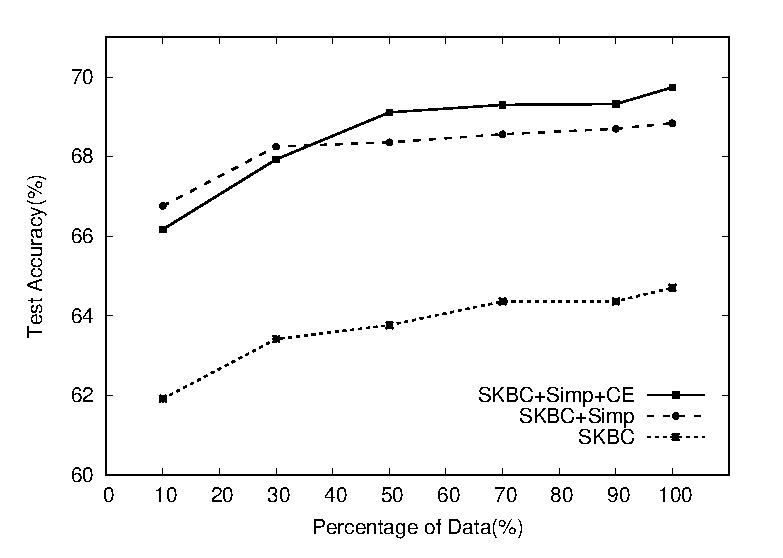
\includegraphics[width=0.8\columnwidth]{pictures/trend}
%\caption{Accuracies over train data size \KZ{Change the notation
%to SS and CG}}\label{fig:trend}
%\end{figure}

%In \figref{fig:trend}, we compare the models' capability with different methods given increasing
%amount of training data (ROCS*(Tr)). The first observation is that 
%\KZ{Simp and CE are not really models. They are just methods to represent
%stories... Be careful with the choice of words and consistency throughout the paper. Consider changing the labels of the lines in Figure 3.}
% our two methods (SS and SS+CG) both perform well even 
%with very little training data. In fact,
%given 10\% of the data, they already achieve higher accuracy than SKBC using
%the whole data. The second observation is that compared with SKBC, model with our methods
 %improves more quickly as the training data grows, which is indicated by
%the steeper slope from 10\% to 50\% of the data. 
%Finally, when comparing the effects with or without the concept embedding, 
%we can see that without structured knowledge,
%the model is unable to take advantage of more training data. 

%\subsection{Training Time}
%\label{sec:time}
%Except for the improvement on end-to-end accuracy, the simplification 
%can also take a one-third reduction in training time.
%The improvement in efficiency comes from fewer tokens in sentences 
%and smaller vocabulary.
% \eve{what is 'various of data'? 'various' should be 'variousness'}
%There are 43,095 unique words in all ROCStories and 
%19,455 unique words in simplified key tokens extracted from ConceptNet. 
%This greatly reduces the vocabulary size.
%In addition, the structured commonsense feature 
%also brings in extra commonsense knowledge. 
%the best result for WSE is 64.7\% with all data. 
%Though accuracy is still growing, the growth is slowing down. 
%With the limited training data, our model performs much better. 
%The reducing of noise and variance improves sentence representation quality. 
%The concepts embedding from , though can't give all the sentence information to the representation, helps improve the accuracy to 69.7\% which is the state of art in model comparison. The results suggest neither of these two kind of sentence embedding is sufficient to represent the commonsense knowledge and the combination can give the best performance.
